\documentclass[10pt,letterpaper]{article}
\usepackage[utf8]{inputenc}
\usepackage{amsmath}
\usepackage{amsfonts}
\usepackage{amssymb}
\usepackage{graphicx}
\usepackage{enumerate}
\usepackage{verbatim}
\usepackage{subfig}
\usepackage{gensymb}
\graphicspath{ {ReportImages/} }
\providecommand{\e}[1]{\ensuremath{\times 10^{#1}}}
\usepackage[left=2cm,right=2cm,top=2cm,bottom=2cm]{geometry}
\author{Michael Smith, Haisin Yip, Yang Zhou}
\title{ECSE 415 Project Report}
\begin{document}
\maketitle

\textbf{Part 1}
\vspace{5mm}
\paragraph{}
Figs. \ref{training1}, \ref{training2} and \ref{training3} are examples of all the possible poses for a given subject.  These include yaw rotations from -45\degree,-30\degree,0\degree,30\degree and 45\degree at 3 different scales: close, medium and far.  The images were taken on a white background.
\paragraph{}
Figs. \ref{testing1}, \ref{testing2} and \ref{testing3} show the different testing poses for a given subject.  These include all of the rotations of the training images with the subject facing upwards followed by facing downwards.  In addition, different images were taken of each subject without their glasses, with different facial expressions and with a hat on.

\vspace{5mm}
\textbf{Part 2}
\paragraph{}
Fig. \ref{part2sift} shows 10 selected faces with their SIFT features. Note some faces are blurry as the images are low resolution to allow for acceptable computation time although some subjects are far away.
\paragraph{}
Fig. \ref{part2lbphist} shows three examples of region histograms for a given training image.  We can see that the tendency is for the lower values to have greater frequency.
\paragraph{}
Fig. \ref{part2codewords} shows four histograms.  They represent two images; each image has its histogram representing the codewords computed for both LBP and SIFT.

\vspace{5mm}
\textbf{Part 3}
\paragraph{}
Fig. \ref{part3classify} shows five examples of classification using both LBP and SIFT. We see that some images, such as (b) or (c) are correctly classified but others such as (e) are not.

\paragraph{}
With respect to the performance of the classifier, SIFT performs the best with a recognition rate of  69.6429\% with K = 20.  This is likely due to the fact that SIFT is more robust to the changes in lighting (mostly due to the iPhone's sensitivity to indirect light when pictures at a greater distance were taken) and scale seen in the training images as well as the testing images.  LBP performs about as well as flipping a coin, although considering the variations in the images this is to be expected.
\paragraph{}
Finally, Fig. \ref{part4} shows five group photos with the faces detected and tagged.  Overall, the performance is quite poor.  In (a), while all the faces are detected they are all incorrect.  In (b), Haisin is correctly detected on the left but not on the right where the algorithm believes him to be a clone of Haisin.  Similarly, Eric is correctly detected in the center but somehow is duplicated on Michael behind him.  In (c), Eric us correctly detected albeit with an extremely large bounding box. None of the other members are detected.  In (d), the only person to be detected is detected incorrectly. In (e), Gavin is correctly detected but not Haisin, who is misidentified as Michael.

It is likely that the poor performance of the algorithm with respect to the group photos is due to the fact that the lighting conditions and poses vary dramatically, far exceeding the poses and variations in the training images.
\begin{figure}[p]
\centering
\subfloat[]{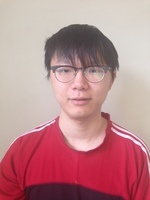
\includegraphics[width = 0.2\textwidth]{Training/gavin_close_0_133_122_32_19.jpg}}
\subfloat[]{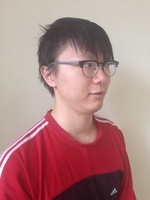
\includegraphics[width = 0.2\textwidth]{Training/gavin_close_30_30_15_124_121.jpg}}
\subfloat[]{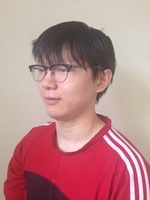
\includegraphics[width = 0.2\textwidth]{Training/gavin_close_-30_126_21_20_124.jpg}}
\subfloat[]{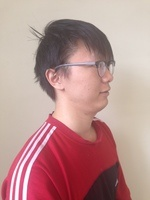
\includegraphics[width = 0.2\textwidth]{Training/gavin_close_45_24_18_118_120.jpg}}
\subfloat[]{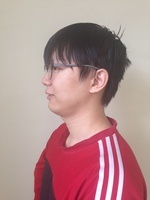
\includegraphics[width = 0.2\textwidth]{Training/gavin_close_-45_31_22_130_122.jpg}}
\caption{Training images at the close, medium and far scales.}
\label{training1}
\end{figure}

\begin{figure}[p]
\centering
\subfloat[]{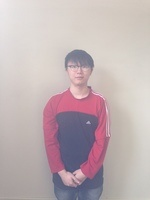
\includegraphics[width = 0.2\textwidth]{Training/gavin_medium_0_57_46_101_90.jpg}}
\subfloat[]{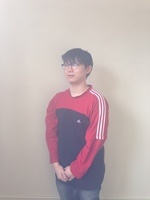
\includegraphics[width = 0.2\textwidth]{Training/gavin_medium_-30_54_47_97_88.jpg}}
\subfloat[]{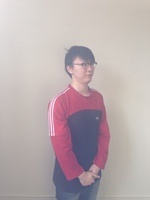
\includegraphics[width = 0.2\textwidth]{Training/gavin_medium_30_106_44_58_84.jpg}}
\subfloat[]{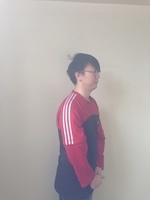
\includegraphics[width = 0.2\textwidth]{Training/gavin_medium_45_58_50_107_93.jpg}}
\subfloat[]{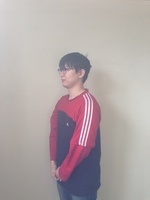
\includegraphics[width = 0.2\textwidth]{Training/gavin_medium_-45_96_50_51_90.jpg}}
\caption{Training images at the medium scale.}
\label{training2}
\end{figure}

\begin{figure}[p]
\centering
\subfloat[]{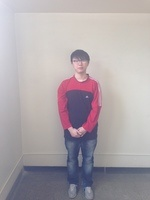
\includegraphics[width = 0.2\textwidth]{Training/gavin_far_0_98_48_63_74.jpg}}
\subfloat[]{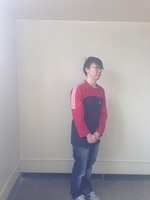
\includegraphics[width = 0.2\textwidth]{Training/gavin_far_30_75_54_109_85.jpg}}
\subfloat[]{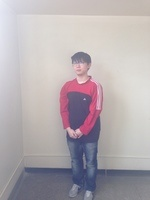
\includegraphics[width = 0.2\textwidth]{Training/gavin_far_-30_96_50_66_78.jpg}}
\subfloat[]{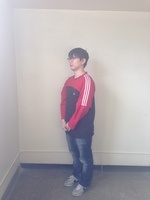
\includegraphics[width = 0.2\textwidth]{Training/gavin_far_-45_60_46_93_75.jpg}}
\subfloat[]{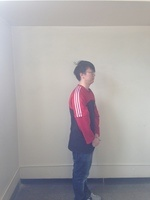
\includegraphics[width = 0.2\textwidth]{Training/gavin_far_45_104_60_68_88.jpg}}
\caption{Training images at the far scale.}
\label{training3}
\end{figure}

\begin{figure}[p]
\centering
\subfloat[]{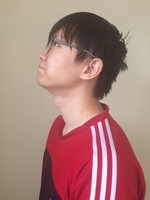
\includegraphics[width = 0.2\textwidth]{Testing/gavin_close_-45_up_134_13_31_118.jpg}}
\subfloat[]{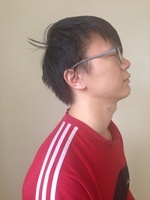
\includegraphics[width = 0.2\textwidth]{Testing/gavin_close_45_up_31_21_144_124.jpg}}
\subfloat[]{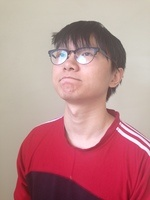
\includegraphics[width = 0.2\textwidth]{Testing/gavin_close_-30_up_37_22_130_118.jpg}}
\subfloat[]{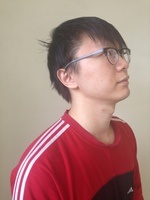
\includegraphics[width = 0.2\textwidth]{Testing/gavin_close_30_up_34_19_143_119.jpg}}
\subfloat[]{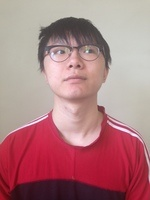
\includegraphics[width = 0.2\textwidth]{Testing/gavin_close_0_up_30_19_122_120.jpg}}
\caption{Testing images of the subject with their head facing upwards.}
\label{testing1}
\end{figure}

\begin{figure}[p]
\centering
\subfloat[]{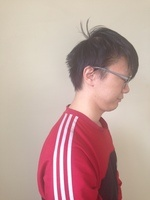
\includegraphics[width = 0.2\textwidth]{Testing/gavin_close_45_down_58_33_139_120.jpg}}
\subfloat[]{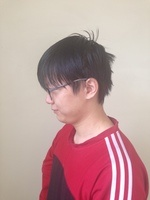
\includegraphics[width = 0.2\textwidth]{Testing/gavin_close_-45_down_25_44_128_129.jpg}}
\subfloat[]{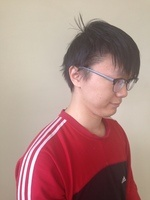
\includegraphics[width = 0.2\textwidth]{Testing/gavin_close_30_down_146_22_54_126.jpg}}
\subfloat[]{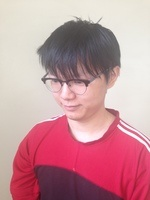
\includegraphics[width = 0.2\textwidth]{Testing/gavin_close_-30_down_29_29_127_120.jpg}}
\subfloat[]{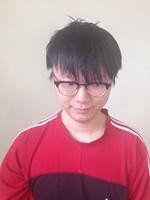
\includegraphics[width = 0.2\textwidth]{Testing/gavin_close_0_down_131_23_41_124.jpg}}
\caption{Testing images of the subject with their head facing downwards.}
\label{testing2}
\end{figure}

\begin{figure}[p]
\centering
\subfloat[]{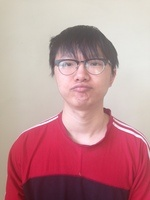
\includegraphics[width = 0.25\textwidth]{Testing/gavin_close_0_smile2_40_25_126_124.jpg}}
\subfloat[]{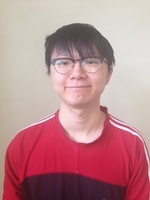
\includegraphics[width = 0.25\textwidth]{Testing/gavin_close_0_smile1_36_26_124_126.jpg}}
\subfloat[]{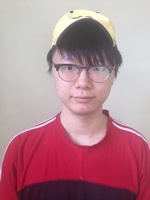
\includegraphics[width = 0.25\textwidth]{Testing/gavin_close_0_hat_38_14_127_128.jpg}}
\subfloat[]{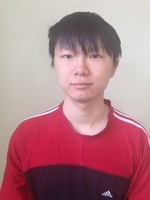
\includegraphics[width = 0.25\textwidth]{Testing/gavin_close_0_glasses_128_16_42_119.jpg}}
\caption{Testing images of the subject with accessories and different facial expressions.}
\label{testing3}
\end{figure}

%% Part 2
\begin{figure}[p]
\centering
\subfloat[]{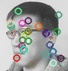
\includegraphics[width = 0.1\textwidth]{SIFT/siftimage0.jpg}}
\subfloat[]{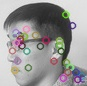
\includegraphics[width = 0.1\textwidth]{SIFT/siftimage1.jpg}}
\subfloat[]{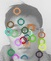
\includegraphics[width = 0.1\textwidth]{SIFT/siftimage2.jpg}}
\subfloat[]{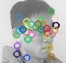
\includegraphics[width = 0.1\textwidth]{SIFT/siftimage3.jpg}}
\subfloat[]{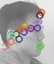
\includegraphics[width = 0.1\textwidth]{SIFT/siftimage4.jpg}}
\subfloat[]{
\includegraphics[width = 0.1\textwidth]{SIFT/siftimage5.jpg}}
\subfloat[]{
\includegraphics[width = 0.1\textwidth]{SIFT/siftimage6.jpg}}
\subfloat[]{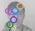
\includegraphics[width = 0.1\textwidth]{SIFT/siftimage7.jpg}}
\subfloat[]{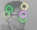
\includegraphics[width = 0.1\textwidth]{SIFT/siftimage8.jpg}}
\subfloat[]{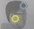
\includegraphics[width = 0.1\textwidth]{SIFT/siftimage9.jpg}}

\caption{SIFT Features for 10 selected faces.}
\label{part2sift}
\end{figure}

\begin{figure}[p]
\centering
\subfloat[]{
\includegraphics[width = 0.30\textwidth]{LBPHist/LBP_Hist_1.jpg}}
\hspace{5mm}
\subfloat[]{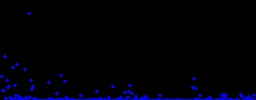
\includegraphics[width = 0.30\textwidth]{LBPHist/LBP_Hist_2.jpg}}
\hspace{5mm}
\subfloat[]{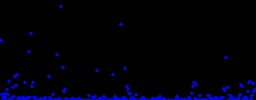
\includegraphics[width = 0.30\textwidth]{LBPHist/LBP_Hist_3.jpg}}

\caption{Three examples of region histograms for a given training image.}
\label{part2lbphist}
\end{figure}

\begin{figure}[p]
\centering
\subfloat[LBP for Image 1]{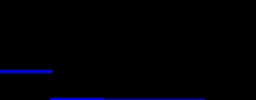
\includegraphics[width = 0.20\textwidth]{CodeWordHist/LBP_Hist_1.jpg}}
\hspace{5mm}
\subfloat[LBP for Image 2]{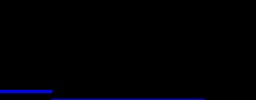
\includegraphics[width = 0.20\textwidth]{CodeWordHist/LBP_Hist_2.jpg}}
\hspace{5mm}
\subfloat[SIFT for Image 1]{
\includegraphics[width = 0.20\textwidth]{CodeWordHist/SIFT_Hist_1.jpg}}
\hspace{5mm}
\subfloat[SIFT for Image 2]{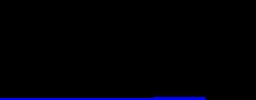
\includegraphics[width = 0.20\textwidth]{CodeWordHist/SIFT_Hist_2.jpg}}

\caption{Histograms representing the codewords for SIFT and LBP for two select images.}
\label{part2codewords}
\end{figure}

\begin{figure}[p]
\centering
\subfloat[LBP]{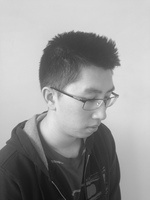
\includegraphics[width = 0.15\textwidth]{Part3Classify/lbp_20_classify_38_supposedtobe_gavin.jpg}}
\hspace{5mm}
\subfloat[LBP]{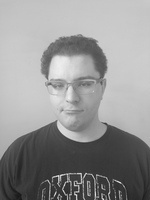
\includegraphics[width = 0.15\textwidth]{Part3Classify/lbp_20_classify_50_supposedtobe_michael.jpg}}
\hspace{5mm}
\subfloat[SIFT]{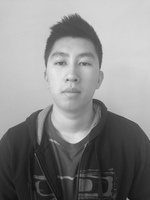
\includegraphics[width = 0.15\textwidth]{Part3Classify/sift_20_classify_33_supposedtobe_haisin.jpg}}
\hspace{5mm}
\subfloat[SIFT]{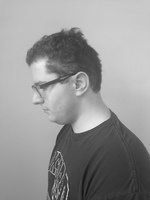
\includegraphics[width = 0.15\textwidth]{Part3Classify/sift_20_classify_44_supposedtobe_michael.jpg}}
\hspace{5mm}
\subfloat[LBP]{\includegraphics[width = 0.15\textwidth]{Part3Classify/lbp_20_classify_9_supposedtobe_michael.jpg}}

\caption{Five examples of classification using both LBP and SIFT. (a) is classified as Gavin when it is in fact Haisin. (b) is classified correctly as Michael.  (c) is classified correctly as Haisin.  (d) is classified correctly as Michael.  (e) is classified as Michael but is in fact Eric.}

\label{part3classify}
\end{figure}

\begin{figure}[p]
\centering
\subfloat[]{\includegraphics[width = 0.3\textwidth]{Part4/0.jpg}}
\hspace{2mm}
\subfloat[]{\includegraphics[width = 0.3\textwidth]{Part4/1.jpg}}
\hspace{2mm}
\subfloat[]{\includegraphics[width = 0.3\textwidth]{Part4/2.jpg}}
\hspace{2mm}
\subfloat[]{\includegraphics[width = 0.3\textwidth]{Part4/3.jpg}}
\hspace{2mm}
\subfloat[]{\includegraphics[width = 0.3\textwidth]{Part4/4.jpg}}

\caption{Five group photos with faces detected and tagged.}

\label{part4}
\end{figure}

\end{document}